\documentclass[12pt]{jarticle}
\usepackage{TUSIReport}
\usepackage{otf}
\usepackage[dvipdfmx]{graphicx}
\usepackage[dvipdfmx]{color}
\usepackage{amsmath}
\usepackage{amssymb}
\usepackage{color}
\usepackage{hhline}
\usepackage{fancybox,ascmac}
\usepackage{multirow}
\usepackage{url}
\usepackage{bm}
\usepackage{listings,jlisting}
\lstdefinestyle{log}{
    frame={tblr},
    basicstyle={\footnotesize},
    tabsize={4},
}
\lstdefinestyle{lstcpp}{
    language={c++},
    backgroundcolor={\color[gray]{.85}},
    basicstyle={\small},
    identifierstyle={\small},
    commentstyle={\small\ttfamily \color[rgb]{0,0.5,0}},
    keywordstyle={\small\bfseries \color[rgb]{1,0,0}},
    ndkeywordstyle={\small},
    stringstyle={\small\ttfamily \color[rgb]{0,0,1}},
    frame={tb},
    breaklines=true,
    columns=[l]{fullflexible},
    numbers=left,
    xrightmargin=0zw,
    xleftmargin=3zw,
    numberstyle={\scriptsize},
    stepnumber=1,
    numbersep=1zw,
    morecomment=[l]{//}
}
\begin{document}
%%%%%%%%%%%%%%%%%%%%%%%%%%%%%%%%%%%%%%%%%%%%%%%%%%%%%%%%%%%%%%
% 表紙を出力する場合は,\提出者と\共同実験者をいれる
% \提出者{科目名}{課題名}{提出年}{提出月}{提出日}{学籍番号}{氏名}
% \共同実験者{一人目}{二人目}{..}{..}{..}{..}{..}{八人目}
%%%%%%%%%%%%%%%%%%%%%%%%%%%%%%%%%%%%%%%%%%%%%%%%%%%%%%%%%%%%%%
\提出者{情報工学実験2}{実験テーマ3 情報通信シミュレーション}{2020}{12}{14}{4619055}{辰川力駆}
\共同実験者{}{}{}{}{}{}{}{}

%%%%%%%%%%%%%%%%%%%%%%%%%%%%%%%%%%%%%%%%%%%%%%%%%%%%%%%%%%%%%%
% 表紙を出力しない場合は,以下の「\表紙出力」をコメントアウトする
%%%%%%%%%%%%%%%%%%%%%%%%%%%%%%%%%%%%%%%%%%%%%%%%%%%%%%%%%%%%%%
\表紙出力

%%%%%%%%%%%%%%%%%%%%%%%%%%%%%%%%%%%%%%%%%%%%%%%%%%%%%%%%%%%%%%
% 以下はレポート本体である.別途 TeXファイルを作成し \input 使っても良い
%%%%%%%%%%%%%%%%%%%%%%%%%%%%%%%%%%%%%%%%%%%%%%%%%%%%%%%%%%%%%%

\section{実験概要}
ハミング符号を用いたシミュレーションプログラムを作成し、
誤り率を求め、グラフを参考にしながら、情報通信の特性や原理を理解する。

\section{目的}
通信システムの「シミュレーション」を通し、
ディジタル通信システムと誤り訂正符号の理解を深める。
ここでは、コンピューター・シミュレーションと呼ばれるもので、
コンピューター上で仮想的な通信環境を構築し実験を行うものである。

\section{原理}

\subsection{誤り訂正符号}

情報を伝えるとき、できるだけ正確に伝えるための仕組みである。
送信メッセージに $N − K$ ビットの冗長性をもたせることで、
通信路で発生した誤りを訂正することが可能である。

\begin{itemize}
    \item 符号化 (Encode)

          送信者は $K$ ビットの送りたい情報 $\boldsymbol{w}$ をルールに従って
          $N$ ビットの符号語 $\boldsymbol{x}$ に変換する。
    \item 復号 (Decode)

          受信者は $\boldsymbol{x}$ がわからず、
          ノイズ付きの情報 $\boldsymbol{y}$ のみを知っている。
          $\boldsymbol{y}$ から $\hat{\boldsymbol{x}}$ および $\hat{\boldsymbol{w}}$ を推定する。
\end{itemize}

\begin{figure}[h]
    \begin{center}
        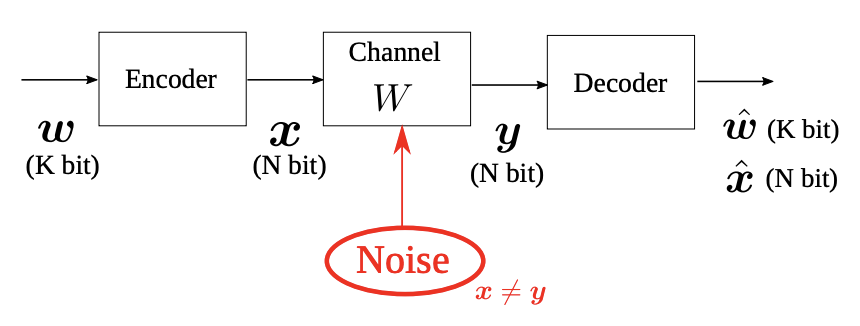
\includegraphics[scale=0.5]{kadai3_3_2.png}
    \end{center}
    \caption{通信路モデル}
\end{figure}

\clearpage

\subsection{ハミング符号}

ハミング符号はブロック符号の一種である。
デジタル情報をブロック ($K$ ビット) に分け、
それぞれに対して符号化を行う (N ビットになる)。
\begin{figure}[h]
    \begin{center}
        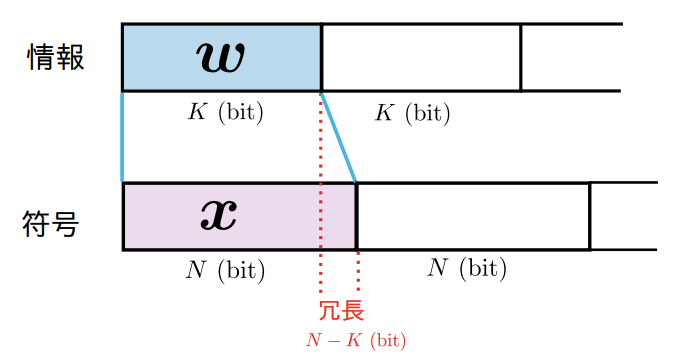
\includegraphics[scale=0.5]{kadai3_3_1.png}
    \end{center}
    \caption{ブロック符号化}
\end{figure}

\section{実験手順}
\begin{enumerate}
    \item $K=4$ビットの情報 $\boldsymbol{w}$ を乱数を用いて生成
    \item 符号化により、$\boldsymbol{w}$ から $\boldsymbol{x}$ を生成
    \item 乱数を用いて$N=7$ビットの雑音ベクトル $\boldsymbol{e}$ を生成
    \item $\boldsymbol{y}=\boldsymbol{x}\oplus \boldsymbol{e}$ を計算
    \item $\boldsymbol{y}$ から復号して$\hat{\boldsymbol{x}}$、$\hat{\boldsymbol{w}}$ を得る
    \item $\boldsymbol{w}$と$\hat{\boldsymbol{w}}$を比較し、ビット誤り数をカウント
    \item 1から6をSIM回行い、ビット/ブロック誤り率を計算
\end{enumerate}

\clearpage

\section{実験結果}

ソースコードは付録に記述した。
そのソースコードを実行した結果を下記に示す。

なお、誤り率を$\epsilon=0.005,0.009,0.013,0.017,0.021$、
シミュレーション回数を$\rm{SIM}=1000000$に設定した。

また、これらの結果をグラフにプロットした。

\begin{figure}[h]
    \begin{center}
        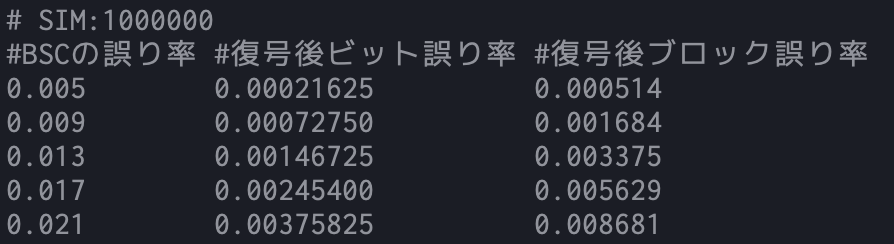
\includegraphics[scale=0.5]{kadai3_3_3.png}
    \end{center}
    \caption{ソースコードの実行結果}
\end{figure}

\begin{figure}[h]
    \begin{center}
        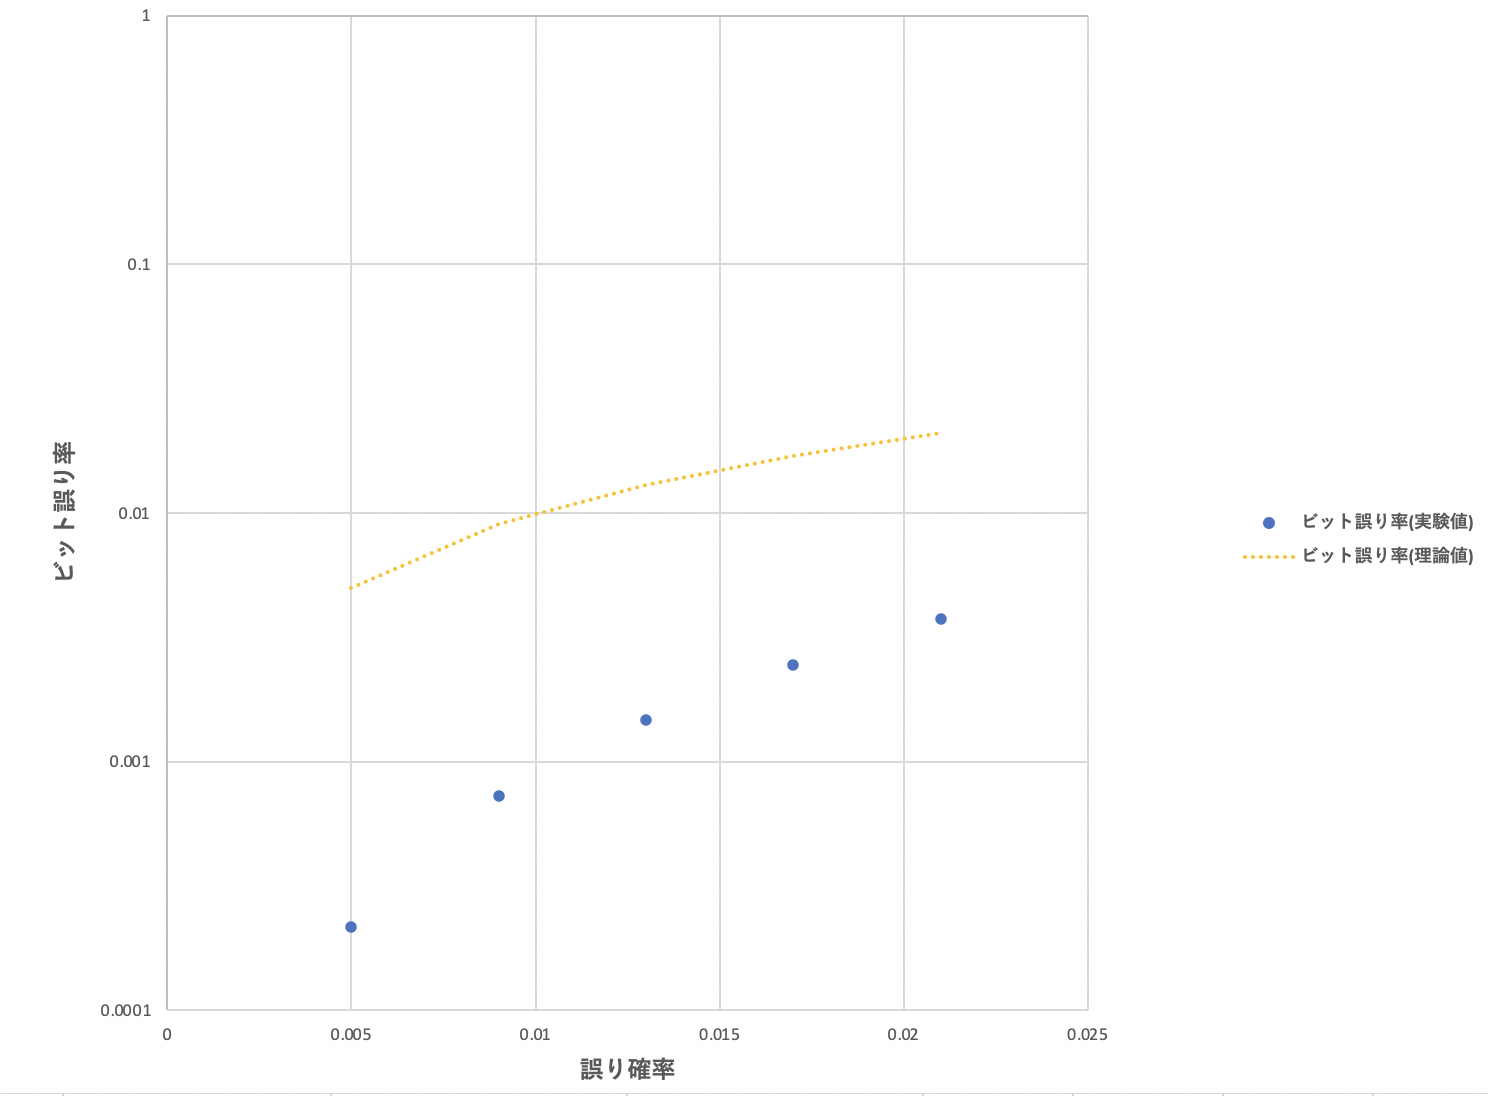
\includegraphics[scale=0.25]{kadai3_3_4.png}
    \end{center}
    \caption{ビット誤り率のグラフ}
\end{figure}

\clearpage

\begin{figure}[h]
    \begin{center}
        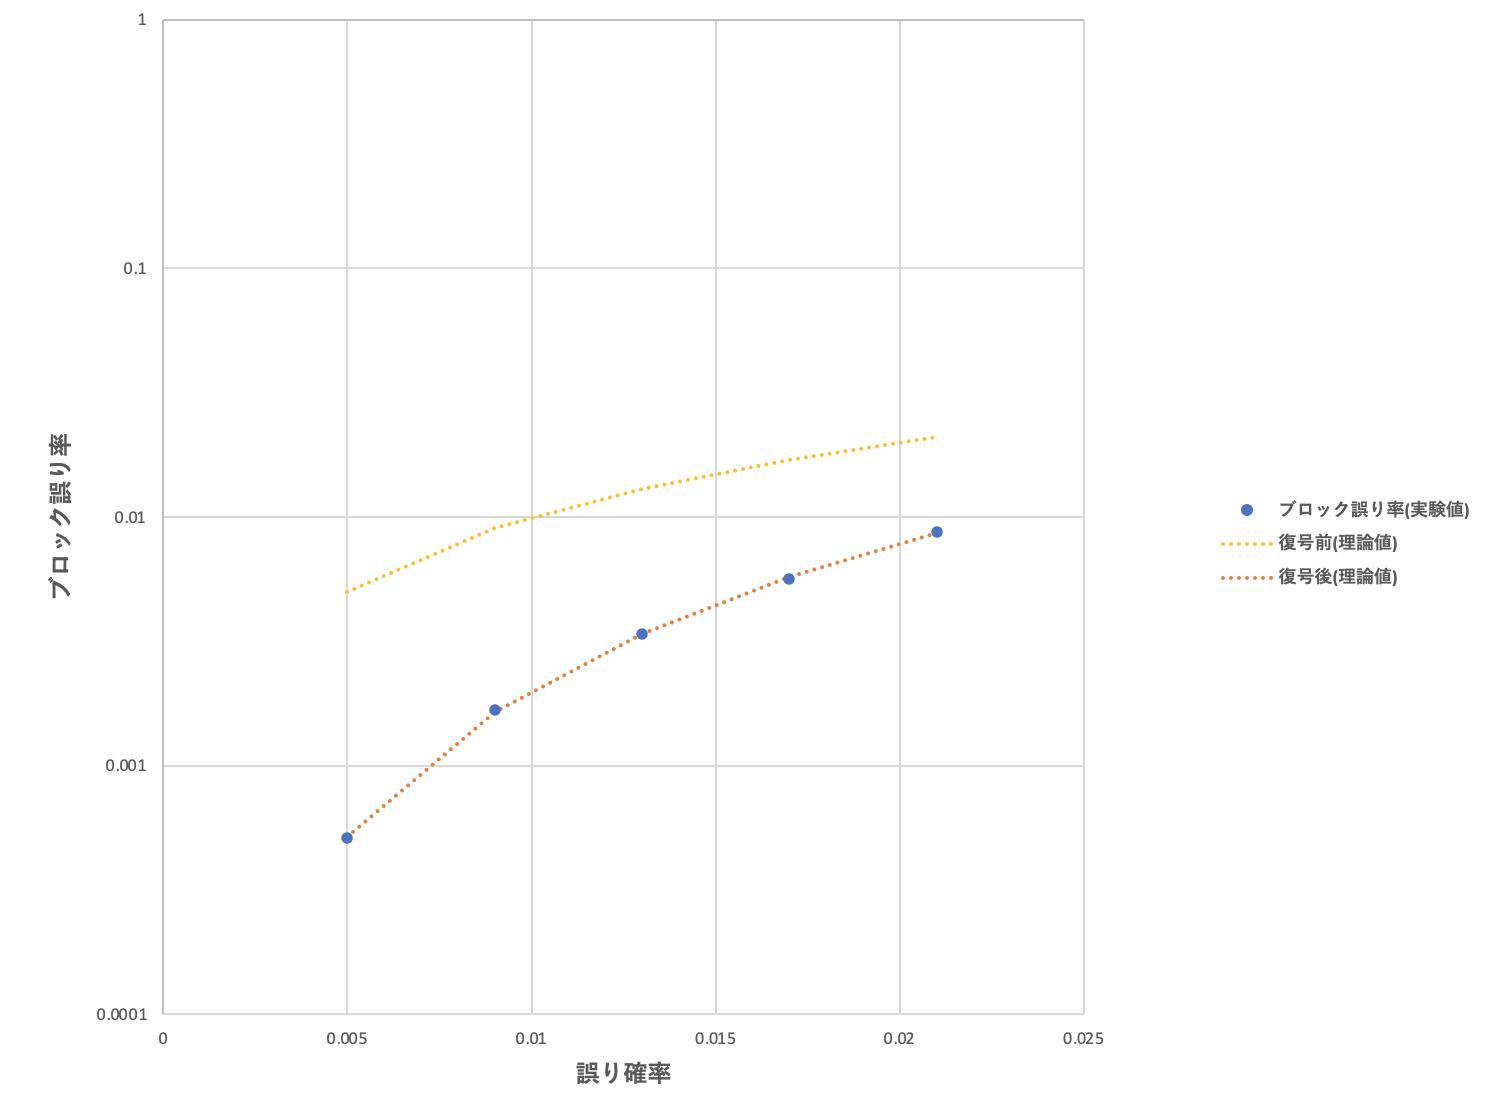
\includegraphics[scale=0.25]{kadai3_3_5.png}
    \end{center}
    \caption{ブロック誤り率のグラフ}
\end{figure}

\section{検討}
\subsection{課題1}
\begin{shadebox}
    $\epsilon$を非常に小さくした場合 ($10^{-4}$ 程度)、
    誤り率を正しく測定するためにはどの程度のシミュレーション回数が必要か。
\end{shadebox}

\subsection{課題2}
\begin{shadebox}

\end{shadebox}

\subsection{課題3}
\begin{shadebox}

\end{shadebox}

\clearpage
% 付録
\appendix
\section{付録}
\begin{lstlisting}[style = lstcpp,caption=kadai3\_3.cpp]
    //4619055 辰川力駆
    #include <random> // 乱数生成
    #include <stdio.h>
    #include <iostream>
    #include <iomanip>
    
    using namespace std;
    
    #define N 7         ///符号化後のビット数
    #define K 4         ///デジタル情報の分けるブロックのビット数
    #define seed 55     ///学籍番号下2桁
    #define SIM 1000000 ///シミュレーション回数
    
    mt19937 mt(seed); ///メルセンヌ・ツイスタ
    
    int main()
    {
        uniform_real_distribution<double> rand_real(0, 1);
        normal_distribution<double> rand_n(0, 0.3);
    
        int w[K];                  //4ビットの情報w
        int x[N];                  //7ビットの符号語x
        int e[N];                  //7ビットの雑音ベクトルe
        int y[N];                  //7ビットの受信語y
        int s[3];                  ///シンドロームs
        int bit_count = 0;         ///シミュレーションごとの毎回のビット誤り数を計算
        int total_bit_count = 0;   ///誤ったビットの総数
        int total_block_count = 0; ///ブロック単位の誤りの総数
        int EstimationPosition;    ///誤り位置推定場所
        double ep;                 ///誤り率
    
        cout << "# SIM:" << SIM << endl;
        cout << "#BSCの誤り率 #復号後ビット誤り率 #復号後ブロック誤り率" << endl;
    
        for (int k = 0; k < 5; k++)
        {
            ep = 0.005 + k * 0.004;
            total_bit_count = 0;
            total_block_count = 0;
    
            for (int sim = 0; sim < SIM; sim++)
            {
                bit_count = 0;
    
                for (int i = 0; i < K; i++) //K=4 ビットの情報 w を乱数を用いて生成
                {
                    w[i] = rand_real(mt) * 2;
                }
    
                for (int i = 0; i < K; i++) ///符号化により, w から x を生成
                {
                    x[i] = w[i];
                }
                x[N - K + 1] = w[0] ^ w[1] ^ w[2];
                x[N - K + 2] = w[1] ^ w[2] ^ w[3];
                x[N - K + 3] = w[0] ^ w[1] ^ w[3];
    
                for (int i = 0; i < N; i++) ///乱数を用いてN=7ビットの雑音ベクトルeを生成
                {
                    if (rand_real(mt) <= ep)
                    {
                        e[i] = 1;
                    }
                    else
                    {
                        e[i] = 0;
                    }
                }
    
                for (int i = 0; i < N; i++) //xとeの排他的論理和を計算してyとする
                {
                    y[i] = x[i] ^ e[i];
                }
    
                s[0] = y[0] ^ y[1] ^ y[2] ^ y[4]; //yから復号してxハット、wハットを得る
                s[1] = y[1] ^ y[2] ^ y[3] ^ y[5];
                s[2] = y[0] ^ y[1] ^ y[3] ^ y[6];
    
                int point = 0;
                for (int i = 0; i < 3; i++)
                {
                    point += s[i] * pow(2, 2 - i);
                }
                switch (point)
                {
                case 5:
                    EstimationPosition = 1;
                    break;
                case 7:
                    EstimationPosition = 2;
                    break;
                case 6:
                    EstimationPosition = 3;
                    break;
                case 3:
                    EstimationPosition = 4;
                    break;
                case 4:
                    EstimationPosition = 5;
                    break;
                case 2:
                    EstimationPosition = 6;
                    break;
                case 1:
                    EstimationPosition = 7;
                    break;
                default:
                    EstimationPosition = -1;
                    break;
                }
                if (EstimationPosition != -1)
                {
                    y[EstimationPosition - 1] = y[EstimationPosition - 1] ^ 1;
                }
    
                for (int i = 0; i < K; i++) //w と wハットを比較し、 ビット誤り数をカウント(つまり4ビットまでを見れば良い)
                {
                    bit_count += w[i] ^ y[i];
                }
    
                total_bit_count += bit_count;
    
                if (bit_count != 0)
                {
                    total_block_count += 1;
                }
            }
            cout << ep;
            cout << fixed << setprecision(8) << "        " << (double)total_bit_count / (K * SIM);
            cout << fixed << setprecision(6) << "          " << (double)total_block_count / SIM << endl;
            cout.unsetf(ios::fixed); ///体裁を整えている
        }
        return 0;
    }
    
\end{lstlisting}

%%%%%%%%%%%%%%%%%%%%%%%%%%%%%%%%%%%%%%%%%%%%%%%%%%%%%%%%%%%%%%
\end{document}